\section{Experiment}

\subsection{Experimental Implementation}

Conventional Naive Bayes implementations stores a structure the size of \\
\\
$|Features| * |Label|$ \\
\\
in memory. In our classification case, this would be a \\
\\
$(|Subject\_Categories|+|Unique\_Subject|\\+|Object\_Categories|+|Object\_Subject|) * |Verbs|$ \\

sized structure. This is unfeasible for the amount of data we are working with. To deal with such a large volume of data we proposed a Naive Bayes algorithm in MapReduce implemented in Hadoop. This method of Naive Bayes is similar to Streaming Naive Bayes and does not require large global structures to be kept.\\
\\
At a high level, this requires going over the data 4 times. Once to count the number of occurrences of each verb. Once to count the number of occurrences of each Subject, Object and their categorical counts. Once to train. Once to test and evaluate the results. At the end of each phase, we store some small statistics into the context of our map and reduce jobs such as the number of unique subjects, objects, ontology for the next task.\\
\\
We only need to transform counts into conditional probabilities in the testing phase, since conditional probabilities are only needed for each test example. We can do a map emitting $<$Subject\/Object, [TestNum, test\_counts, train\_counts]$>$. This way we can parallelize to the full extent by putting all necessary information to calculate conditional probabilities in the reducer for a given Subject or Object. 

\subsection{Result Comparison}

\subsubsection{Comparison between categorical smoothing and Laplace smoothing}

\begin{table}[t]
\caption{Precision Comparison between categorical smoothing and Laplace smoothing}
\label{tab-smoothing-comparison}
\vskip 0.15in
\begin{center}
\begin{small}
\begin{sc}
\begin{tabular}{l|cc|c}
\hline
\abovespace\belowspace
Data set & Laplace & categorical & improvement \\
\hline
\abovespace
Top 1k set & 0.5906 & 0.8764 & 0.2858 \\
\belowspace
Lower 1k set & 0.6455 & 0.8128 & 0.1673 \\
\hline
\end{tabular}
\end{sc}
\end{small}
\end{center}
\vskip -0.1in
\end{table}

We use two different verb sets to compare the effect of categorical smoothing and Laplace smoothing. One set is the top 1000 most frequent unstemmed verbs in the SVO tuple corpus, the other lower 1000 set is the 10001st to 11000th most frequent unstemmed verbs in the SVO tuple corpus. The top 1000 set contains 538 unique stemmed verbs while the lower 1000 set contains 935 unique stemmed verbs. However, the number of examples in training and testing set are quite different. The top 1000 set has about 206k testing examples while the lower 1000 set has 18.9k testing examples. The numbers of training set have the same proportion.

From the comparison result in \ref{tab-smoothing-comparison}, we see that categorical smoothing provides a significant improvement on the precision on both datasets. It improves the precision on top 1000 set for 0.2858 and lower 1000 set for 0.1673 respectively. We also observe that the improvement of categorical smoothing is more significant on the top 1000 set than on the lower 1000 set.

\subsection{Comparison between Unigram Prior and Uniform Prior}

\begin{table}[t]
\caption{Precision Comparison between Unigram Prior and Uniform Prior}
\label{tab-prior-comparison}
\vskip 0.15in
\begin{center}
\begin{small}
\begin{sc}
\begin{tabular}{l|cc}
\hline
\abovespace \belowspace
Data set & Top 100 set & Lower 100 set \\
\hline
\abovespace
unigram prior & 0.8603 & 0.6376 \\
\belowspace
uniform prior & 0.9314 & 0.7784 \\
\hline
\abovespace
\belowspace
Difference & 0.0711 & 0.1408 \\
\hline
\end{tabular}
\end{sc}
\end{small}
\end{center}
\vskip -0.1in
\end{table}

\subsection{Smoothing Parameter}

\begin{figure}[ht]
\vskip 0.2in
\begin{center}
\centerline{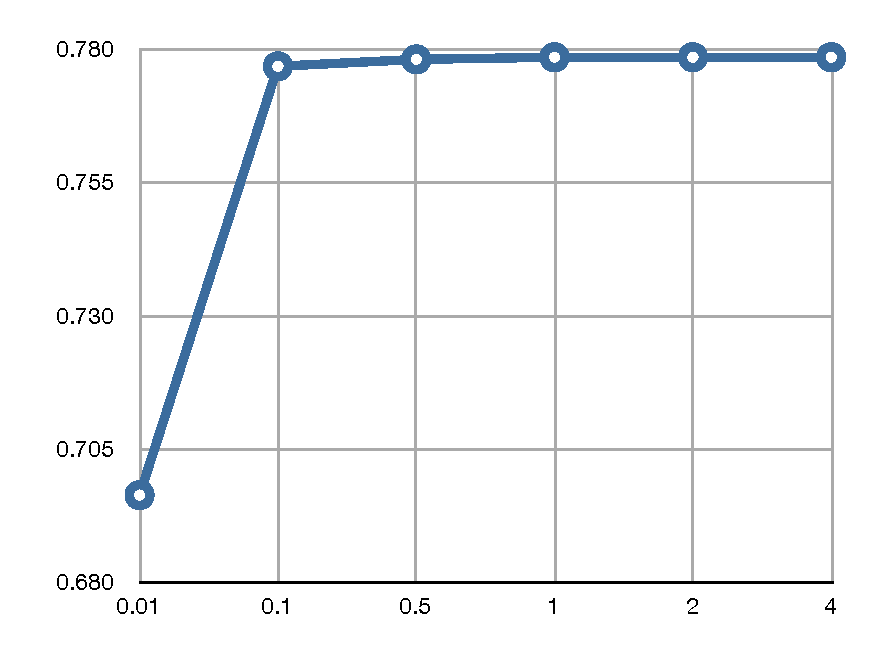
\includegraphics[width=\columnwidth]{pvsalpha}}
\caption{Precision vs. Smoothing parameter in Categorical Smoothing}
\label{fig-p-vs-alpha}
\end{center}
\vskip -0.2in
\end{figure}

We tune the smoothing parameter $alpha$



